\section{Aufgaben und Durchführung}
\label{sec:Durchführung}
\subsection{Bestimmung der Zeitkonstante}
In der ersten Aufgabe soll die Zeitkonstante eines RC-Gliedes bestimmt werden.
Dies geschieht mit dem Aufbau nach Abbildung \ref{abb:schaltbildRC}
\begin{figure}[h]
    \centering
    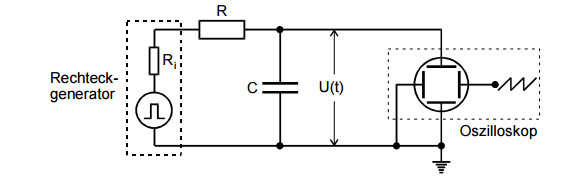
\includegraphics[width=0.7\textwidth]{aufbaua.PNG}
    \caption{Schaltbild zur bestimmung der RC-Konstante.\cite{skript}}
    \label{abb:schaltbildRC}
\end{figure}\\
Am Generator wird eine Rechteckspannung erzeugt, die entsprechende Kondensatorspannug $U_C(t)$ wird auf das Oszilloskop gegeben.
Zur bestimmung der Zeitkonstante wird entweder die Auflade-oder Entladekurve betrachtet und Wertepaare von $U_C$ und $t$ aufgenommen.
\subsection{Messung der Amplitude}
In der zweiten Aufgabe ist nach der Amplitude der Kondensatorspannung in Abhängigkeit von der Frequenz der generierten Spannung gefragt.
Zur Bestimmung dieser wird die Schaltung aus Abbildung \ref{abb:schaltbildAmplitude} benutzt.
\begin{figure}[h]
    \centering
    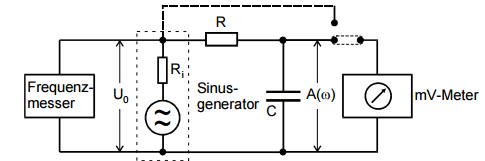
\includegraphics[width=0.7\textwidth]{aufbaub.PNG}
    \caption{Schaltbild zur bestimmung der Kondensatorspannungsamplitude.\cite{skript}}
    \label{abb:schaltbildAmplitude}
\end{figure}
\newpage
Der Generator erzeugt in diesem Aufgabenteil eine Sinusspannung und die Amplitude der entsprechenden Kondensatorspannung wird mit einem Voltmeter vermessen.
Die Messung geht über drei Zehnerpotenzen der Frequenz der Generatorspannung.
Zum Schluss wird eine Frequenzabhängigkeit der Generatorspannung selbst untersucht, dazu wird der Generator am Voltmeter angeschlossen.
\subsection{Messung der Phasenverschiebung}
In der dritten Aufgabe soll die frequenzabhängige Phasenverschiebung zwischen Generator-und Kondensatorspannung untersucht.
Um die Phasenverschiebung zu bestimmen werden Generator und Kondensatorspannung am Oszilloskop dargestellt,
wie im schematischen Aufbau in Abbildung \ref{abb:schaltbildPhase} zu erkennen.
\begin{figure}[h]
    \centering
    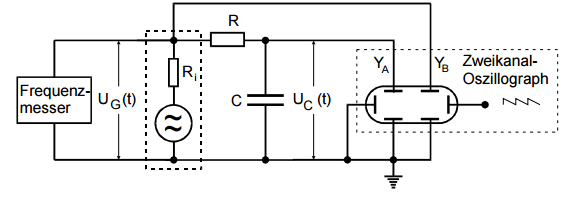
\includegraphics[width=0.7\textwidth]{aufbaucd.PNG}
    \caption{Schaltbild zur bestimmung der Phasenverschiebung und Eignung als Integrator.\cite{skript}}
    \label{abb:schaltbildPhase}
\end{figure}\\
Mit der Cursor Funktion am Oszilloskop wird der Abstand $a$ der beiden Nulldurchgänge und die Schwingungsdauer $b$ abgelesen, dies geschieht für verschiedene Frequenzen,
wie in Abbildung \ref{abb:Phase} zu sehen.
\begin{figure}[h]
    \centering
    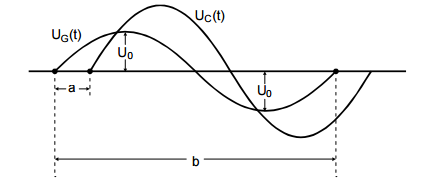
\includegraphics[width=0.7\textwidth]{messungc.PNG}
    \caption{Beispielbild für den Messvorgang der Phasenverschiebung.\cite{skript}}
    \label{abb:Phase}
\end{figure}\newpage
\subsection{Eignung als Integrator}
In der vierten Aufgabe soll gezeigt werden, dass das RC-Glied für bestimmte Frequenzen als Integrator fungiert.
Hierzu wird der Aufbau nach Abbildung \ref{abb:schaltbildPhase} genutzt. Am Generator werden Sinus-, Rechteck und Dreiecksspannung eingestellt, mit einer Frequenz größer als $\frac{1}{RC}$ ist.
Thermodrücke von der Kondensatorspannung werden mittels Oszilloskop aufgenommen.
